\begin{ex}%Câu 1
	Trong KG $Oxyz$ gọi $(P)\colon ax+by+cz-3=0$ ($a$,$b$,$c$ là các số nguyên không đồng thời bằng $0$) là phương trình mặt phẳng đi qua hai điểm $M(0;-1;2)$, $N(-1;1;3)$ và không đi qua $H(0;0;2)$. Biết rằng khoảng cách từ $H(0;0;2)$ đến mặt phẳng $(P)$ đạt giá trị lớn nhất. Tính giá trị của $P=a-2b+3c+12$. 
	\shortans{$16$}
\loigiai{
	Mặt phẳng $(P)$ đi qua hai điểm $M(0;-1;2),N(-1;1;3)$ nên ta có\\
	 $\heva{
			&7-b+2c-3=0\\
			&-a+b+3c-3=0
		}\Rightarrow\heva{
				&b=2c-3\\
				&a=5c-6.
		}$ $(*)$\\
	Mặt khác $\mathrm{d}(H;(P))=\dfrac{|2c-3|}{\sqrt{a^2+b^2+c^2}}.$ $(**)$\\
	Thay $(*)$ vào $(**)$ ta được $\mathrm{d}(H;(P))=\dfrac{|2c-3|}{\sqrt{a^2+b^2+c^2}}=\dfrac{|2c-3|}{\sqrt{30c^2-72c+45}}$.\\
	Xét hàm số $y=\dfrac{2c-3}{\sqrt{30c^2-72c+45}}$ có tập xác định $\mathscr{D}=\mathscr{R}$.\\
	$y'=\dfrac{18c-18}{30c^2-72c+45}$;\quad$y'=0 \Leftrightarrow  c=1 \Rightarrow y=-\dfrac{1}{\sqrt {3}}$\\
	và $\displaystyle\lim_{c\to +\infty}y =\dfrac{2}{\sqrt{30}}$;$\displaystyle\lim_{c\to +\infty}y=-\dfrac{2}{\sqrt{30}}$ $\Rightarrow \min\limits_{x\in\mathscr D}y =y(1)=-\dfrac{1}{\sqrt 3}$.\\
	Xét hàm số $g(c)=\dfrac{|2c-3|}{\sqrt{30c^2-72c+45}}$.\\
	Từ đó suy ra $\max\limits_{\mathscr {D}} g(c)=f(1)=\dfrac{1}{3}$ đạt tại $c=1$.\\
	Với $c=1\Rightarrow a=-1;b=-1$.\\
	Vậy $P=a-2b+3c+12=16$.}
	\end{ex}

	\begin{ex}%Câu 2
Trong KG $Oxyz$ Mặt phẳng $(P)$ đi qua điểm $M(1;1;1)$ cắt các tia $Ox$, $Oy$, $Oz$ lần lượt tại $A(a;0;0)$, $B(0;b;0)$, $C(0;0;c)$ sao cho thể tích khối tứ diện $O.ABC$ nhỏ nhất. Tính $T=a+2b+3c$.
\shortans{$18$}
\loigiai{
Từ giả thiết ta có $a > 0$, $b > 0$, $c > 0$ và thể tích khối tứ diện $O.ABC$ là $V_{O.ABC}=\dfrac{1}{6}abc$.\\
Ta có phương trình đoạn chắn mặt phẳng $(P)$ có dạng $\dfrac{x}{a}+\dfrac{y}{b}+\dfrac{z}{c}=1$.\\
Mà $M\in(P)\Rightarrow\dfrac{1}{a}+\dfrac{1}{b}+\dfrac{1}{c}=1$.\\
Áp dụng bất đẳng thức Côsi cho ba số ta có $1=\dfrac{1}{a}+\dfrac{1}{b}+\dfrac{1}{c} \geq 3\sqrt[3]{\dfrac{1}{abc}}\Rightarrow abc\geq 27$.\\
Do đó $V_{O.ABC}=\dfrac{1}{6}abc\ge\dfrac{9}{2}$. Đẳng thức xảy ra khi và chỉ khi $a=b=c=3$.\\
Vậy $\min_{V_{O.ABC}}=\dfrac{9}{2}\Leftrightarrow a=b=c=3$. Khi đó $T=a+2b+3c=18$.}
\end{ex}

\begin{ex}%Câu 3
Trong KG $Oxyz$, cho điểm $M(1;4;9)$. Gọi $(P)$ là mặt phẳng đi qua $M$ và cắt 3 tia $Ox$, $Oy$, $Oz$ lần lượt tại các điểm $A$, $B$, $C$ (khác $O$) sao cho $OA+OB+OC$ đạt giá trị nhỏ nhất. Tính khoảng cách $d$ từ gốc tọa độ $O$ đến mặt phẳng $(P)$ (làm tròn đến hàng phần trăm).
\shortans{$5{,}14$}
\loigiai{
Giả sử $A(a;0;0)$, $B(0;b;0)$, $C(0;0;c)$ với $a,b,c > 0$.\\
Phương trình mặt phẳng $(P)\colon\dfrac{x}{a}+\dfrac{y}{b}+\dfrac{z}{c}=1$.\\
$M(1;4;9)\in(P)\Rightarrow\dfrac{1}{a}+\dfrac{4}{b}+\dfrac{9}{c}=1$.\\
Áp dụng BĐT Bunhiacopxki
\begin{eqnarray*}
\left (\dfrac{1}{a}+\dfrac{4}{b}+\dfrac{9}{c}\right)(a+b+c)	& = & \left(\left(\sqrt{\dfrac{1}{a}}\right)^2+\left(\sqrt{\dfrac{4}{b}}\right)^2+\left(\sqrt{\dfrac{9}{c}}\right)^2\right)((\sqrt a)^2+(\sqrt b)^2+(\sqrt c)^2)\\
	&\geq & {(1+2+3)^2}.
	\end{eqnarray*}
		$\Rightarrow  a+b+c\geq 49$.\\
Dấu “$=$ ” xảy ra khi$\heva{&\dfrac{1}{a}+\dfrac{4}{b}+\dfrac{9}{c}=1\\&\dfrac{1}{a}=\dfrac{2}{b}=\dfrac{3}{c}}\overset{a+b+c=49}{\longrightarrow}\heva{&a=6\\&b=12\\&c=18.}$\\
Nên $(P)\colon\dfrac{x}{6}+\dfrac{y}{12}+\dfrac{z}{18}=1$.\\
Vậy $d=\dfrac{36}{7}\approx5{,}14$.}
\end{ex}

\begin{ex}%Câu 4
Trong KG $Oxyz$, mặt phẳng $(P)$ đi qua điểm $M(1;2;1)$ cắt các tia $Ox$, $Oy$, $Oz$ lần lượt tại các điểm $A$, $B$, $C$ ($A$, $B$, $C$ không trùng với gốc $O$) sao cho tứ diện $O.ABC$ có thể tích nhỏ nhất. Viết phương trình mặt phẳng $(P)\colon\dfrac{x}{a}+\dfrac{y}{b}+\dfrac{z}{c}=1$. Tính $T=a+b+c$.
\shortans{$12$}
\loigiai{
Gọi $(P)$ cắt các tia $Ox$, $Oy$, $Oz$ lần lượt tại các điểm $A(a;0;0)$; $B(0;b;0)$; $C(0;0;c)$ $(a,b,c > 0)$.\\
Ta có $(P)\colon\dfrac{x}{a}+\dfrac{y}{b}+\dfrac{z}{c}=1$.\\
Vì $M\in(P)$ nên ta có $\dfrac{1}{a}+\dfrac{2}{b}+\dfrac{1}{c}=1$.\\
Áp dụng bất đẳng thức Côsi ta có $1=\dfrac{1}{a}+\dfrac{2}{b}+\dfrac{1}{c}\geq\dfrac{3\sqrt[3]{2}}{\sqrt[3]{abc}}\Rightarrow abc\geq 54$.\\
Thể tích khối chóp $V_{O.ABC}=\dfrac{1}{6}abc\geq 9$.\\
Dấu bằng xảy ra khi các số tham gia Côsi bằng nhau nghĩa là\\
 $\heva{
&\dfrac{1}{a}+\dfrac{2}{b}+\dfrac{1}{c}=1\\
&\dfrac{1}{a}=\dfrac{2}{b}=\dfrac{1}{c}
}\Leftrightarrow \heva{&a=3\\&b=6\\&c=3.}$\\
Vây phương trình mặt phẳng $(P)\colon\dfrac{x}{3}+\dfrac{y}{6}+\dfrac{z}{3}=1\Rightarrow a+b+c=12$.}
\end{ex}

\begin{ex}%Câu 5
Trong KG $Oxyz$, cho ba điểm $A(a;0;0)$, $B(0;b;0)$, $C(0;0;c)$, trong đó $a$, $b$, $c$ là các số thực thỏa mãn $\dfrac{2}{a}-\dfrac{2}{b}+\dfrac{1}{c}=1$. Tính khoảng cách từ gốc tọa độ $O$ đến mặt phẳng $(ABC)$.
\shortans{$3$}
\loigiai{
Phương trình mặt phẳng $(ABC)\colon\dfrac{x}{a}+\dfrac{y}{b}+\dfrac{z}{c}=1$.\\
Nhận thấy, điểm $M(2;-2;1)\in(ABC)$ ; $\overrightarrow{OM}=(2;-2;1)$, $OM=3$.\\
Ta có $\mathrm{d}(O;(ABC))=OH\leq OM$. \\
$\Rightarrow $  $\mathrm{d}(O;(ABC))$ có giá trị lớn nhất khi $OM\perp (ABC)$ $\Leftrightarrow \overrightarrow{n_{(ABC)}}=k\cdot\overrightarrow{OM},(k\neq 0)$. \\
$\Rightarrow\heva{
&\dfrac{1}{a}=2k\\
&\dfrac{1}{b}=-2k\\
&\dfrac{1}{c}=k
}\Rightarrow\heva{
&a=\dfrac{1}{2k}\\
&b=-\dfrac{1}{2k}\\
&c=\dfrac{1}{k}.
}$\\
Mà $\dfrac{2}{a}-\dfrac{2}{b}+\dfrac{1}{c}=1$ nên $\dfrac{2}{\dfrac{1}{2k}}-\dfrac{2}{-\dfrac{1}{2k}}+\dfrac{1}{\dfrac{1}{k}}=1\Leftrightarrow 9k=1\Leftrightarrow k=\dfrac{1}{9}$. \\
Do đó $a=\dfrac{9}{2}$; $b=-\dfrac{9}{2}$; $c=9$.\\
Vậy $\mathrm{d}_{\max}(O;(ABC))=OM=3$ khi $a=\dfrac{9}{2}$; $b=-\dfrac{9}{2}$; $c=9$.}
\end{ex}

\begin{ex}%Câu 6
Trong KG $Oxyz$, cho điểm $M(1;4;9)$. Gọi $(P)$ là mặt phẳng đi qua $M$ và cắt 3 tia $Ox$, $Oy$, $Oz$ lần lượt tại các điểm $A$, $B$, $C$ (khác $O$) sao cho $OA+OB+OC$ đạt giá trị nhỏ nhất. Tính khoảng cách $d$ từ gốc tọa độ $O$ đến mặt phẳng $(P)$ (làm tròn đến hàng phần trăm).
\shortans{$5{,}14$}
\loigiai{
Gọi mặt phẳng $(P)$ đi qua điểm $M(1;4;9)$ cắt các tia $Ox$ tại $A(a;0;0)$, $B(0;b;0)$, $C(0;0;c)$ với $a$, $b$, $c>0$ ta có $(P)\colon\dfrac{x}{a}+\dfrac{y}{b}+\dfrac{z}{c}=1$ suy ra $\dfrac{1}{a}+\dfrac{4}{b}+\dfrac{9}{c}=1$.\\
 Và $OA+OB+OC=a+b+c$ đạt giá trị nhỏ nhất khi\\
$$1=\dfrac{1}{a}+\dfrac{4}{b}+\dfrac{9}{c}=\dfrac{1^2}{a}+\dfrac{2^2}{b}+\dfrac{3^2}{c}\geq\dfrac{(1+2+3)^2}{a+b+c}\Rightarrow a+b+c\geq 36.$$\\
Dấu bằng xảy ra khi và chỉ khi $\heva{
&a=6\\
&b=12\\
&c=18
}$ $\Rightarrow(P)\colon\dfrac{x}{6}+\dfrac{y}{12}+\dfrac{z}{18}=1$.\\
Nên $\mathrm{d}(O;(P))=\dfrac{|\dfrac{0}{6}+\dfrac{0}{12}+\dfrac{0}{18}-1|}{\sqrt{(\dfrac{1}{6})^2+(\dfrac{1}{12})^2+(\dfrac{1}{18})^2}}=\dfrac{36}{7}\approx 5{,}14$.}
\end{ex}

\begin{ex}%Câu 7
Trong KG $Oxyz$, cho ba điểm $A(a,0,0), B(0,b,0), C(0,0,c)$ với $a, b, c$ là những số dương thay đổi thỏa mãn $a^2+4b^2+16c^2=49$. Tính tổng $S=a^2+b^2+c^2$ khi khoảng cách từ $O$ đến mặt phẳng $(ABC)$ đạt giá trị lớn nhất.
\shortans{$12{,}3$}
\loigiai{
Dựng $OH\perp(ABC)$; $(H\in(ABC))$ vì $OABC$ là tứ diện vuông nên ta có
$$\dfrac{1}{OH^2}=\dfrac{1}{OA^2}+\dfrac{1}{OB^2}+\dfrac{1}{OC^2}=\dfrac{1}{a^2}+\dfrac{1}{b^2}+\dfrac{1}{c^2}=\dfrac{1}{a^2}+\dfrac{2^2}{4b^2}+\dfrac{4^2}{16c^2}.$$\\
Áp dụng bất đẳng thức Schwarz
$$\dfrac{1}{OH^2}=\dfrac{1}{a^2}+\dfrac{2^2}{4b^2}+\dfrac{4^2}{16c^2}\geq\dfrac{(1+2+4)^2}{a^2+4b^2+16c^2}=1\Rightarrow OH\leq 1.$$
Vậy khoảng cách từ $O$ đến mặt phẳng $(ABC)$ đạt giá trị lớn nhất là $1$ khi
$$\dfrac{1}{a^2}=\dfrac{2}{4b^2}=\dfrac{4}{16c^2}=\dfrac{1+2+4}{a^2+4b^2+16c^2}=\dfrac{1}{7}\Rightarrow\heva{
&{a^2}=7\\
&{b^2}=\dfrac{7}{2}\\
&{c^2}=\dfrac{7}{4}
}\Rightarrow S=\dfrac{49}{4}\approx12{,}3.$$
}
\end{ex}

\begin{ex}%Câu 8
Trong KG $Oxyz$, cho mặt phẳng $(P)\colon x+y-z+2=0$ và hai điểm $A(3;4;1)$; $B(7;-4;-3)$. Điểm $M(a;b;c)(a > 2)$ thuộc $(P)$ sao cho tam giác $ABM$ vuông tại $M$ và có diện tích nhỏ nhất. Tính giá trị biểu thức $T=a+b+c$.
\shortans{$0$}
\loigiai{
Ta có $S_{ABM}=\dfrac{1}{2}AB.MH$ với $H$ là hình chiếu vuông góc của $M$ lên $AB$.\\
Do $AB$ không đổi nên $S_{ABM}$ nhỏ nhất khi $MH$ nhỏ nhất.\\
$\heva{
&\overrightarrow{AB}=(4;-8;-4)\\
&\overrightarrow{n}_P =(1;1;-1)
}\Rightarrow\overrightarrow{AB}\cdot\overrightarrow{n}_P=0\Rightarrow AB\parallel(P)$.\\
$MH$ nhỏ nhất khi $M$ nằm trên giao tuyến của mặt phẳng $(Q)$ và $(P)$; với $(Q)$ là mặt phẳng chứa $AB$ và vuông góc với mp$(P)$.\\
$\heva{
&\overrightarrow{AB}=(4;-8;-4)\\
&\overrightarrow{n}_P=(1;1;-1)
}\Rightarrow\overrightarrow{n}_Q=(3;0;3)\Rightarrow $ phương trình mặt phẳng $(Q)$ là $x+z-4=0$.\\
$M$ nằm trên giao tuyến của mặt phẳng $(Q)$ và $(P)$ nên tọa độ $M$ là nghiệm của hệ phương trình $\heva{
&x+z-4=0\\
&x+y-z+2=0
}\Rightarrow\heva{
&x=t\\
&y=2-2t\\
&z=4-t
}\Rightarrow M(t;2-2t;4-t)$ với $t > 2$.\\
Ta có $\overrightarrow{AM}=(t-3;-2-2t;3-t);\overrightarrow{BM}=(t-7;6-2t;7-t)$.\\
Tam giác $ABM$ vuông tại $M$ nên\\
 $\overrightarrow{AM}\cdot\overrightarrow{BM}=0\Leftrightarrow(t-3)(t-7)+(-2-2t)(6-2t)+(3-t)(7-t)=0$.\\
$\Rightarrow(t-3)(t-7)+2(t-3)(t+1)=0\Rightarrow(t-3)(3t-5)=0\Leftrightarrow\hoac{
&t=3\text{ (nhận)}\\
&t=\dfrac{5}{3}\text{ (loại).}
}$\\
Với $t=3\Rightarrow M(3;-4;1)\Rightarrow a+b+c=3-4+1=0$.}
\end{ex}

\begin{ex}%[2H5C1-3]
	Trong KG $Oxyz$, cho đường thẳng $d\colon \heva{&x=4-3t\\ &y=3+4t\\ &z=0}$. Gọi $A$ là hình chiếu vuông góc của $O$ trên $d$. Điểm $M$ di động trên tia $Oz$, điểm $N$ di động trên đường thẳng $d$ sao cho $MN=OM+AN$. Gọi $I$ là trung điểm đoạn thẳng $OA$. Trong trường hợp diện tích tam giác $IMN$ đạt giá trị nhỏ nhất, phương trình của mặt phẳng chứa điểm $M$ và đường thẳng $d$ có dạng $4x+by+cz+d=0$. Khi đó giá trị $b+c+d$ bằng (làm tròn đến hàng phần trăm).
	\shortans{$0{,}07$}
	\loigiai{
		\begin{center}
			\begin{tikzpicture}[scale=1,line join=round,line cap=round,font=\footnotesize,>=stealth]% coordinates
				\path (0,0) coordinate (A) % theo phép tịnh tiến theo 1 góc.
				++(0:5) coordinate (O) 
				++(90:2.5)  coordinate (M)
				++(-115:6) coordinate (N)
				++(90:2.95) coordinate (I)
				++(-55:1.45) coordinate (H)
				($(N)!1.7!(A)$) coordinate (N')
				($(M)!1.5!(O)$) coordinate (P)
				($(A)!1.5!(N)$) coordinate (A');
				\coordinate (d) at (-1.5,1) ;
				\draw (A)--(O)--(M)--(N)--(I) (N)--(A) (A)--(N') (I)--(H) (O)--(P) (I)--(P)(A')--(N');
				\foreach \x/\y in {A/180,O/0,M/90,N/-145,I/90,H/0,P/-90 %hiện điểm
				}{\draw[fill=black] (\x) circle(1pt)++(\y:0.35)node{$\x$};}%nút tròn ngay điểm
				\path (d)node [right]{$d$};
				\draw pic[draw, angle radius=2.5mm]{right angle=N--A--O}; 
				\draw pic[draw, angle radius=2.5mm]{right angle=A--O--M}; 
			\end{tikzpicture}
		\end{center}
		Gọi $A(4-3t;3+4t;0)$ là hình chiếu vuông góc của $O$ trên $d$\\
		$\Leftrightarrow OA\perp d \Leftrightarrow \overrightarrow{OA} \cdot \overrightarrow{u}_d=0 \Leftrightarrow t=0 \Rightarrow A(4;3;0)$.\\
		Trên $Oz$ lấy điểm $P$ sao cho $OP=AN \Rightarrow MP=OM+OP=MN$\\
		và $\Delta AIN=\Delta OIP \Rightarrow IN=IP$.\\
		Ta có $\Delta IMP=\Delta IMN$, kẻ $IH\perp MN \Rightarrow IH=IO$\\
		$\Rightarrow{S_{\Delta IMN}}=\dfrac{1}{2}IH \cdot MN \Rightarrow{S_{\Delta IMN}} \min \Leftrightarrow MN_{\min}$.\\
		Ta có $MN^2=MO^2+OA^2+AN^2 \ge 2\left(\dfrac{MO+AN}{2}\right)^2+25 \Rightarrow MN \geq 5\sqrt 2$.\\
		Vậy $MN_{\min}=5\sqrt 2 \Leftrightarrow OM=AN=\dfrac{5\sqrt 2}{2} \Rightarrow M\left(0;0;\dfrac{5\sqrt 2}{2}\right)$.\\
		Một vectơ pháp tuyến của mặt phẳng $(M,d)$ là $[\overrightarrow{MA},\overrightarrow{u}_d]=\left(10\sqrt 2 ;\dfrac{15}{\sqrt 2};25\right)$.\\
		Chọn $\overrightarrow n=\left(4;3;5\sqrt 2\right)$.\\
		Khi đó phương trình của mặt phẳng $(M,d) \colon 4x+3y+5\sqrt 2 z-10=0$.\\
		Vậy $b+c+d\approx0{,}07$.
	}
\end{ex}

\begin{ex}%[2H5C2-3]
	Trong KG $Oxyz$, cho điểm $A(1;4;3)$ và mặt phẳng $(P) \colon 2y-z=0$. Biết điểm $B$ thuộc $(P)$, điểm $C$ thuộc $(Oxy)$ sao cho chu vi tam giác $ABC$ nhỏ nhất. Tính giá trị nhỏ nhất đó (làm tròn đến hàng phần trăm).
	\shortans{$8{,}94$}
	\loigiai{
		Gọi $H$ là hình chiếu vuông góc của $A(1;4;3)$ lên mặt phẳng $(Oxy) \Rightarrow H(1;4;0)$.\\
		Gọi $A_1$ là điểm đôi xứng của $A$ qua mặt phẳng $(Oxy)$, ta tìm được $A_1(1;4;-3)$.\\
		Gọi $K$ là hình chiếu vuông góc của $A(1;4;3)$ lên mặt phẳng $(P)$.\\
		Ta có PTĐT $AK \colon \heva{&x=1\\ &y=4+2t\\ &z=3-t.}$\\ Gọi $K(1;4+2t;3-t)\in AK$.\\
		Mặt khác, $K\in (P) \Rightarrow 5t+5=0 \Rightarrow t=-1 \Rightarrow K(1;2;4)$.\\
		Gọi $A_2$ là điểm đôi xứng của $A$ qua mặt phẳng $(P)$ thì $K$ là trung điểm của $ AA_2$.\\
		Ta có $\heva{&x_{A_2}=2x_K-x_A=1\\ &y_{A_2}=2y_K-y_A=0\\ &z_{A_2}=2{x_K}-z_A=5} \Rightarrow A_2(1;0;5)$.\\
		Ta có chu vi tam giác $ABC$ là $P_{\Delta ABC}=AC+AB+BC=A_1C+A_2B+BC\ge {A_1}{A_2}$.\\
		Dấu bằng xảy ra khi $A_1$, $A_2$, $B$, $C$ thẳng hàng.\\
		Suy ra $\left(P_{\Delta ABC}\right)_{\min}=A_1A_2=4\sqrt{5}\approx8{,}94$.
	}
\end{ex}
\Closesolutionfile{ans}
% \indapan{6}{ans/ans-C5B3CD5-KQ}
\begin{dang}{GIÁ TRỊ LỚN NHẤT, GIÁ TRỊ NHỎ NHẤT LIÊN QUAN ĐẾN GÓC}
	\subsubsection{Bài toán 1}
	Trong KG $Oxyz$, cho đường thẳng $d$ và mặt phẳng $(P)$ cắt nhau. Lập phương trình của mặt phẳng $(Q)$ chứa $d$ và tạo với mặt phẳng $(P)$ một góc nhỏ nhất.\\
	\textbf{Phương pháp giải}\\
	\begin{itemize}
		\item \textbf{Cách 1: Phương pháp hình học}\\
		\begin{center}
			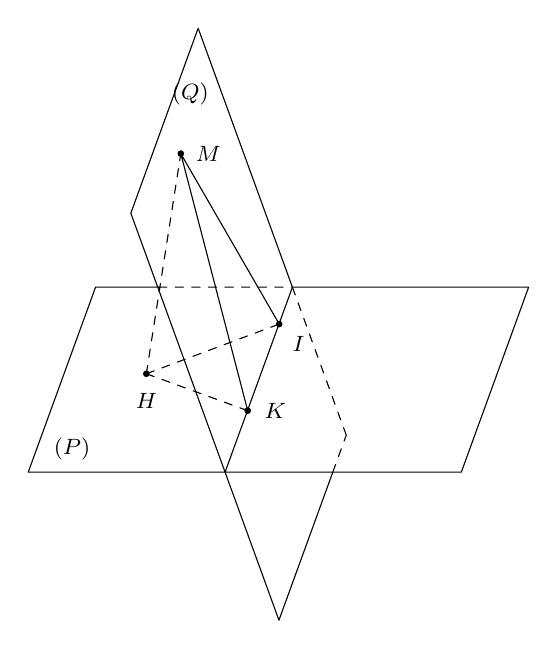
\begin{tikzpicture}[scale=1,line join=round,line cap=round,font=\footnotesize,>=stealth]% coordinates
				\path (0,0) coordinate (A) 
				++(0:2.5) coordinate (A')
				++(0:3) coordinate (B) 
				++(70:2.5)  coordinate (C)
				++(-180:3) coordinate (D)
				++(110:3.5) coordinate (R)
				++(-110:2.5) coordinate (S)
				++(-70:5.5) coordinate (T)
				++(70:2) coordinate (U)
				++(70:0.5) coordinate (W);
				\path (1.5,1.25) coordinate (H) 
				++(-20:1.37) coordinate (K) 
				++(70:1.17)  coordinate (I)
				++(120:2.5) coordinate (M);
				\path (0,0) coordinate (A)
				++(70:2.5) coordinate (E)
				++(0:0.8) coordinate (F);
				\coordinate (P) at (0.2,0.3);
				\coordinate (Q) at (1.7,4.8);
				\draw (A)--(A')--(B)--(C)--(D) (I)--(M)--(K) (A')--(D) (D)--(R)--(S)--(T)--(U) (A)--(E)--(F) ;
				\draw[dashed] (H)--(K) (H)--(I) (H)--(M) (F)--(D) (U)--(W) (D)--(W);
				\foreach \x/\y in {H/-90,K/0,I/-45,M/0 %hiện điểm
				}{\draw[fill=black] (\x) circle(1pt)++(\y:0.35)node{$\x$};}%nút tròn ngay điểm
				\path (P)node [right]{$(P)$};
				\path (Q)node [right]{$(Q)$};
			\end{tikzpicture}
		\end{center}	
		Gọi $I$ là giao điểm của đường thẳng $d$ với mặt phẳng $(P)$ và lấy điểm $M \in d,\, M \ne I$.\\
		Gọi $H$, $K$ lần lượt là hình chiếu của $M$ lên $(P)$ và giao tuyến $\Delta$ của $(P)$ và $(Q)$.\\
		Đặt $\alpha$ là góc giữa $(P)$ và $(Q)$, ta có $\alpha = \widehat{MKH}$, do đó $\tan \alpha =\dfrac{HM}{HK} \ge \dfrac{HM}{HI}$.\\
		Do đó $(Q)$ là mặt phẳng đi qua $d$ và vuông góc với mặt phẳng $(MHI)$, nên $(Q)$ đi qua $M$ và nhận $[[\overrightarrow{n}_P,\overrightarrow{u}_d],\overrightarrow{u}_d]$ làm vectơ pháp tuyến.
		\item \textbf{Cách 2: Phương pháp đại số}\\
		Ta có thể giải bài toán trên bằng phương pháp đại số như sau:\\
		\begin{itemize}
			\item Gọi $\overrightarrow{n}_Q=(a;b;c)$, $(a^2+b^2+c^2 \ne 0)$ là một vectơ pháp tuyến của mặt phẳng $(Q)$.
			\item Khi đó $\overrightarrow{n}_Q \cdot \overrightarrow{u}_d=0$ từ đây ta rút ra được $a$ theo $b$, $c$ (hoặc $b$ theo $a$, $c$ hoặc $c$ theo $a$, $b$).
			\item Gọi $\alpha$ là góc giữa $(P)$ và $(Q)$, ta có $\cos \alpha =\dfrac{|\overrightarrow{n} \cdot \overrightarrow{n}_P|}{|\overrightarrow{n}| \cdot |\overrightarrow{n}_P|}=f(t)$\\
			với $t=\dfrac{b}{c}$, $c \ne 0$. Khảo sát $f(t)$ ta tìm được $\max$ của $f(t)$.
		\end{itemize}
	\end{itemize}
	\begin{note}
		Để tìm vectơ pháp tuyến $\overrightarrow{n}_Q$ của mặt phẳng $(Q)$ đơn giản hơn thì nên gọi $\overrightarrow{n}_Q=(1;b;c)$.
	\end{note}
	
	\subsubsection{Bài toán 2}
	Trong KG $Oxyz$, cho hai đường thẳng $d$ và $d'$ chéo nhau. Viết phương trình mặt phẳng $(P)$ chứa $d$ và tạo với $d'$ một góc lớn nhất.\\
	\textbf{Phương pháp giải}
	\begin{itemize}
		\item \textbf{Cách 1: Phương pháp hình học}\\
		\begin{center}
			\begin{tikzpicture}% coordinates
				\path (0,0) coordinate (O) 
				++(0:6) coordinate (B) 
				++(70:2.5)  coordinate (C)
				++(-180:4) coordinate (D)
				++(-180:1.2) coordinate (E)
				++(-180:0.8) coordinate (F);
				\path (1.5,1.25) coordinate (H)
				++(0:2.5) coordinate (M)
				++(135:3) coordinate (A)
				++(-60:1.5) coordinate (K)
				($(A)!1.5!(M)$) coordinate (M') 
				($(M)!1.5!(A)$) coordinate (A')
				($(K)!2!(M)$) coordinate (M")
				($(M)!1.5!(K)$) coordinate (K");
				\path (5.5,1.25) coordinate (T) 
				++(135:4.5) coordinate (Q);
				\path (5.5,1.25) coordinate (T) 
				++(-45:1.5) coordinate (L);
				\coordinate (P) at (0.2,0.3);
				\coordinate (S) at (0.5,4);
				\coordinate (d) at (5,0.8);
				\coordinate (d') at (2.8,4);
				\draw (O)--(B)--(C)--(D) (H)--(M) (H)--(A) (M)--(A) (E)--(F) (F)--(O) (A)--(A') (M)--(M")(T)--(Q);
				\draw[dashed] (A)--(K) (M)--(K) (H)--(K)(E)--(D) (M)--(M')(K)--(K")(T)--(L);
				\foreach \x/\y in {H/-90,K/-90,A/90,M/45 %hiện điểm
				}{\draw[fill=black] (\x) circle(1pt)++(\y:0.35)node{$\x$};}%nút tròn ngay điểm
				\path (P)node [right]{$(P)$};
				\path (S)node [right]{$\Delta$};
				\path (d)node [right]{$d$};
				\path (d')node [right]{$d'$};
			\end{tikzpicture}
		\end{center}
		\begin{itemize}
			\item Trên đường thẳng $d$, lấy điểm $M$ và dựng đường thẳng $\Delta$ đi qua $M$ song song với $d$.\\
			Khi đó góc giữa $\Delta$ và $(P)$ chính là góc giữa $d$ và $(P)$.
			\item Trên đường thẳng $\Delta$, lấy điểm $A$. Gọi $H$ và $K$ lần lượt là hình chiếu của $A$ lên $(P)$ và $d$, $\alpha$ là góc giữa $\Delta$ và $(P)$.\\
			Khi đó $\alpha = \widehat{AMH}$ và $\cos \alpha =\dfrac{HM}{AM} \ge \dfrac{KM}{AM}$.\\
			Suy ra $(P)$ là mặt phẳng chứa $d$ và vuông góc với mặt phẳng $(AMK)$. Do đó $(P)$ đi qua $M$ và nhận $(\overrightarrow{u}_d \wedge \overrightarrow{u}_d) \wedge \overrightarrow{u}_d$ làm vectơ pháp tuyến.
		\end{itemize}
		\item \textbf{Cách 2: Phương pháp đại số}\\
		Ta có thể giải bài toán trên bằng phương pháp đại số như sau
		\begin{itemize}
			\item Gọi $\overrightarrow{n}_P=(a;b;c)$, $(a^2+b^2+c^2 \ne 0)$ là một VTPT của mặt phẳng $(P)$.
			\item Khi đó $\overrightarrow{n}_p \cdot \overrightarrow{u}_d=0$ từ đây ta rút ra được $a$ theo $b$, $c$ (hoặc $b$ theo $a$, $c$ hoặc $c$ theo $a$, $b$).
			\item Gọi $\alpha$ là góc giữa $(P)$ và $d$, ta có $\sin \alpha = \dfrac{|\overrightarrow{n} \cdot \overrightarrow{u}_d|}{|\overrightarrow{n}| \cdot |\overrightarrow{u}_d|}=f(t)$\\
			với $t=\dfrac{b}{c}$, $c \ne 0$. Khảo sát $f(t)$ ta tìm được $\max$ của $f(t)$.
		\end{itemize}
		\begin{note}
			Để tìm vectơ pháp tuyến $\overrightarrow{n}_P$ của mặt phẳng $(P)$ đơn giản hơn thì nên gọi $\overrightarrow{n}_P=(1;b;c)$.
		\end{note}
	\end{itemize}
\end{dang}
\Closesolutionfile{ans}
\Opensolutionfile{ans}[ans/ans-0-B15-KQ]
\TN
\begin{ex}%[2H5C1-5]
	Trong KG $Oxyz$, cho đường thẳng $d \colon \dfrac{x}{1}=\dfrac{y+1}{-2}=\dfrac{2-z}{1}$. Gọi $(P)$ là mặt phẳng chứa đường thẳng $d$ và tạo với mặt phẳng $(Q) \colon 2x-y-2z-2=0$ một góc có số đo nhỏ nhất. Điểm $A(1;2;3)$ cách mặt phẳng $(P)$ một khoảng bằng
	\choice
	{\True $\sqrt{3}$}
	{$\dfrac{5\sqrt{3}}{3}$}
	{$\dfrac{7\sqrt{11}}{11}$}
	{$\dfrac{4\sqrt{3}}{3}$}
	\loigiai{
		\begin{center}
			\begin{tikzpicture}% coordinates
				\path (0,0) coordinate (O) 
				++(0:6) coordinate (K) 
				++(60:3)  coordinate (P)
				++(-180:3.5) coordinate (Q)
				++(-180:1.1) coordinate (R)
				++(-180:1.4) coordinate (T);
				\path (4,4) coordinate (M)
				++(-77:2.5) coordinate (H)
				++(-180:2.5) coordinate (B)
				++(-40:1.5) coordinate (C)
				++(60:1.3) coordinate (H)
				($(C)!1.5!(B)$) coordinate (C') 
				($(B)!1.5!(C)$) coordinate (B');
				\coordinate (d) at (3.8,0.3);
				\draw (O)--(K)--(P)--(Q) (B)--(C)(H)--(C)(H)--(M)(B)--(C') (B')--(C)(B)--(M)(M)--(C)(R)--(T)(T)--(O);
				\draw[dashed] (H)--(B)(Q)--(R) ;
				\foreach \x/\y in {H/0,B/-180,C/-90,M/90 %hiện điểm
				}{\draw[fill=black] (\x) circle(1pt)++(\y:0.35)node{$\x$};}%nút tròn ngay điểm
				\path (d)node [right]{$\Delta$};
				\draw pic[draw, angle radius=2.5mm]{right angle=H--C--B'};
				\draw pic[draw, angle radius=2.5mm]{right angle=B--C--M};
				\draw pic[draw, angle radius=2.5mm]{right angle=M--H--C}; 
				\draw pic[draw, angle radius=2.5mm]{right angle=M--H--B};   
			\end{tikzpicture}
		\end{center}
		Ta có $d \colon \dfrac{x}{1}=\dfrac{y+1}{-2}=\dfrac{2-z}{1}$ có VTCP $\overrightarrow{u}=(1;-2;-1)$.\\
		$(Q) \colon 2x-y-2z-2=0$ có VTPT $\overrightarrow{n}=(2;-1;-2)$.\\
		Gọi $\alpha$ là góc tạo bởi $d$ và $(Q)$, ta có $\sin \alpha =\left|\cos(\overrightarrow{u},\overrightarrow{n})\right|=\dfrac{\sqrt{6}}{3}$.\\
		Từ hình vẽ, ta có $(d,(P))=\widehat{MBH}$ và $((P),(Q))=\widehat{MCH}$.\\
		Ta thấy $\sin \widehat{MCH}=\dfrac{MH}{MC} \ge \dfrac{MH}{MB}=\dfrac{\sqrt{6}}{3}$.\\
		Vậy góc $((P),(Q))=\widehat{MCH}$ nhỏ nhất khi $\sin \widehat{MCH}=\dfrac{\sqrt{6}}{3}$ hay $\cos \widehat{MCH}=\dfrac{\sqrt{3}}{3}$.\\
        Viết phương trình mặt phẳng $(P)$\\
		\begin{itemize}
			\item \textbf{Cách 1}\\
			Mặt phẳng $(P) \colon Ax+By+Cz+D=0$.\\
			Ta có $\heva{&\overrightarrow{n}_(Q) \cdot \overrightarrow{u}=0\\ &\cos(\overrightarrow{n},\overrightarrow{n}_(Q))=\dfrac{\sqrt{3}}{3}} 
			\Leftrightarrow \heva{&A-2B-C=0\\ &\dfrac{|2A-B-2C|}{3\sqrt{A^2+B^2+C^2}}=\dfrac{\sqrt{3}}{3}}\\
			\Leftrightarrow \heva{&A=2B+C\\ &|3B|=\sqrt{3(2B+C)^2+B^2+C^2}} \Leftrightarrow \heva{&A=2B+C\\ &6B^2+6C^2+12BC=0. \qquad(1).}$\\
			Nếu $B=0$ suy ra $A=C=0$ loại.\\
			Nếu $B\ne 0$ từ $(1)$ suy ra $\left( \dfrac{C}{B}\right) ^2+2\dfrac{C}{B}+1=0 \Leftrightarrow \dfrac{C}{B}=-1 \Rightarrow C=-B$ suy ra $A=B$.\\
			Mặt phẳng $(P) \colon Bx+By-Bz+D=0$ đi qua điểm $N(0;-1;2) \in d$ suy ra $D=3B$.\\
			Vậy phương trình mặt phẳng $(P) \colon x+y-z+3=0$. Suy ra $d(A;(P))=\sqrt{3}$.
			\item \textbf{Cách 2}\\
			Gọi $\Delta=(P) \cap (Q)$ thì góc giữa $(P)$ và $(Q)$ nhỏ nhất khi và chỉ khi $\Delta \perp d$.\\
			Do đó, mặt phẳng $(P)$ thỏa đề bài là mặt phẳng chứa $d$ và cắt $(Q)$ theo giao tuyến $\Delta$ sao cho $\Delta \perp d$.\\
			$\heva{&\Delta \subset (Q)\\ &\Delta \perp d} \Rightarrow \Delta$ nhận $\overrightarrow{u}_\Delta=\left[ \overrightarrow{u}_d,\overrightarrow{n}_(Q)\right] $ làm vectơ chỉ phương.\\
			$(Q)$ chứa $d$ và $\Delta$ $\Rightarrow (P)$ qua $M(0;-1;2) \in d$ và nhận $\overrightarrow{n}=\left[ \overrightarrow{u}_d,\overrightarrow{u}_\Delta\right] =(6;6;-6)$ làm vectơ pháp tuyến $\Rightarrow(P) \colon x+y-z+3=0$.\\
			Vậy $d(A;(P))=\sqrt{3}$.
		\end{itemize}
	}
\end{ex}
